\documentclass[11pt]{article}
%%%%%%%%%%%%%%%%%%%%%%%%%%%%%%%%%%%%%%%%
\usepackage{amsmath}
\usepackage{verbatim}
\usepackage[usenames,dvipsnames]{color}
\usepackage{setspace}
\usepackage{lscape}
\usepackage{longtable}
\usepackage[top=1.25in,bottom=1.25in,left=1in,right=1in]{geometry}
\usepackage{graphicx}
\usepackage{epstopdf}
\usepackage[usenames,dvipsnames]{pstricks}
\usepackage{epsfig}
\usepackage{pstricks-add}
\usepackage{pst-node}
\usepackage{pst-plot}
\usepackage{fancyhdr}
\usepackage[absolute,showboxes]{textpos}
\usepackage{booktabs}
\usepackage{dcolumn}
\usepackage{arydshln}
\usepackage{natbib}
\usepackage{tabularx}
\usepackage{subfigure}

{\newcommand{\districts}{  28,475}
{\newcommand{\provinces}{   2,282}
{\newcommand{\countries}{     151}
 % commands for counts of observations


\newtheorem{proposition}{Proposition}
\newtheorem{corollary}{Corollary}

\setcounter{MaxMatrixCols}{10}
\newcolumntype{d}[1]{D{.}{.}{-2.#1}}
\newenvironment{proof}[1][Proof]{\noindent\textbf{#1.} }{\ \rule{0.5em}{0.5em}}
\setlength{\columnsep}{.2in}
\psset{unit=1cm}

\def\sym#1{\ifmmode^{#1}\else\(^{#1}\)\fi}

\begin{document}
\begin{titlepage}
\vspace{2in} \noindent {\large \today}

\vspace{.5in} \noindent {\Large \textbf{\strut How Tight are Malthusian Constraints?}}

\vspace{.25in} \noindent {\large T. Ryan Johnson}

\vspace{.05in} \noindent University of Houston

\vspace{.25in} \noindent {\large Dietrich Vollrath}

\vspace{.05in} \noindent University of Houston

\vfill \noindent \textsc{Abstract} \hrulefill

\vspace{.05in} \noindent We use rural density and inherent agricultural productivity data from 35,451 districts around the world to estimate the elasticity of agricultural output with respect to land in different agro-climatic regions. The estimated elasticity is highest in regions suitable for temperate agriculture, and lowest in areas suitable for tropical agriculture. We show theoretically that the higher temperate elasticity implies a tighter Malthusian constraint, meaning a greater sensitivity of non-agricultural employment and income per capita to shocks in population size and productivity. Evidence from the post-war mortality transition in developing countries confirms these predictions.

\vspace{.1in} \hrule

\vspace{.5in} \noindent {\small JEL Codes: O1, O13, O44, Q10}

\vspace{.1in} \noindent {\small Keywords: land constraints, Malthusian stagnation, agriculture}

\vspace{.1in} \noindent {\small Contact information: 201C McElhinney Hall, U. of Houston, Houston, TX 77204, devollrath@uh.edu. We thank Francesco Caselli, Martin Fiszbein, Oded Galor, Nippe Lagerl{\"o}f, Debin Ma, Stelios Michalopolous, Nathan Nunn, {\"O}mer {\"O}zak, Enrico Spolaore, Joachim Voth, and David Weil, as well as seminar participants at the London School of Economics, the Brown Conference on Deep-rooted Determinants of Development, and the University of Houston brown bag series for their comments. All errors remain our own.}
\end{titlepage}

\pagebreak 

\section{Introduction}
\onehalfspacing 
A common assumption in studying historical or contemporary development is that a finite (or inelastic) resource, agricultural land, is necessary for production. This ``Malthusian constraint'' implies that, \textit{ceteris paribus}, living standards decline with the absolute size of the population. While this effect may be small for developed nations today, for the heavily agricultural countries of history and today, this Malthusian constraint is (or was) quite salient.\footnote{Combining this constraint with a positive relationship of living standards and population growth yields the canonical Malthusian model of stagnation \citep{ashraf2010dynamics}, and forms the basis for models of the transition from stagnation to sustained growth. The literature on the transition has grown large enough that it is difficult to provide a reasonable summary in a footnote. An overview of this unified growth literature can be found in \citet{Galor:2011uq}, who cites several key contributions \citep{gw00,galor2002natural,Hansen:2002fk,doepke2004accounting,cs2005,lagerlof2006,craftsmills2009,strulik2008population}. Explanations for the Great Divergence in income per capita are often framed in terms of these unified growth models \citep{kp2001,galor2008trading,vollrath2011,vv08,vv13,cs2015}. The Malthusian constraint features in quantitative work on contemporary developing countries that rely on agriculture \citep{Gollin:2007oq,Restuccia:2008hc,weilwilde2009,Gollin:2010ys,ev2016clim}, and is relevant for long-run growth in rich countries due to possible limits to resources \citep{perettovalente2015}.} The sensitivity of living standards to population size depends on the elasticity of agricultural output with respect to agricultural land; the larger the elasticity, the stronger the effect. By itself, knowing this elasticity allows us to quantify the effects of population and productivity on living standards. But beyond that, \textit{variation} in this elasticity across countries or geographic regions implies that there is variation in the ability of population and productivity to alter living standards, with consequences for the study of growth and development. 

In this paper we derive an empirical specification for estimating this elasticity by developing a model of production with agricultural land that expands on standard one-sector Malthusian models. First, we consider an economy that is made up of many locations, each with its own stock of agricultural land, but where labor and other inputs move freely between those locations. This reveals a simple cross-sectional relationship between the density of agricultural workers in a location and agricultural total factor productivity (TFP), and we can recover a direct estimate of the elasticity from this relationship. Second, we allow for the presence of factors beyond just land and labor (e.g. capital), and show that our estimation strategy does not rely on data on these other inputs. Third, we allow for a non-agricultural sector that employs labor. This shows that the spatial relationship of \textit{agricultural} workers and agricultural TFP holds regardless of the aggregate level of agricultural employment or overall development. The spatial distribution of agricultural workers across districts \textit{within} provinces or states is informative about the elasticity of agricultural output with respect to land. We do not have to rely on cross-country comparisons, nor do we have to assume that the elasticity is homogeneous within countries or across agro-climatic zones.

We assemble data at the district level (i.e. 2nd level administrative units within countries) for rural population density in the year 2000 from \citet{hyde31}, and combine that with an measure of the caloric yield in districts built on the data from \citet{galorozak2016}. As in their work, our measure is built on agro-climatic constraints plausibly unaffected by human activity (e.g. soil quality and length of growing season) from the Global Agro-Ecological Zone (GAEZ) project \citep{gaez}, combined with information on the calorie content of various crops. We aggregate the grid cell caloric yields to the district level as our measure of inherent agricultural TFP.

In the end, we have a dataset of\districts \ districts, coming from\provinces \ provinces in\countries \ countries. Using this data, we provide estimates of the elasticity of agricultural output with respect to land for different geographic regions. For districts that are suitable for temperate agriculture, we estimate an elasticity of 0.228 in our baseline specification, a ``tight'' land constraint. In contrast, in districts suitable for tropical tropical agriculture, the estimated elasticity is 0.132, a ``loose'' constraint. The approximate 0.10 difference in elasticity between agriculture types holds up across different definitions of temperate/tropical, and holds whether we exclude heavily urbanized districts, exclude districts from the developed world, or exclude districts within the lower tail of rural density. In all cases the difference is statistically significant.

These differences are repeated with climate types. We estimate the elasticities by climate zone and find that equatorial areas, and those with dry winters and/or monsoonal precipitation, tend to have low elasticities, while temperate and cold areas, and those with regular year-round rainfall, have higher elasticities. This results in variation in the land constraint across political regions of the world. Among the tightest constraints we find are those for Europe (estimated elasticities between 0.259 and 0.287), the U.S. and Canada (0.203), and Northern Africa (0.249). In comparison, South and Southeast Asia (0.152), tropical Africa (0.089), and the tropical Americas (0.113) have the loosest land constraints. 

The estimated size of the elasticities, and their patterns across agriculture type, climate zone, and region are robust across a variety of specifications. All estimates include controls for the percent of a district that is urban, as well as the density of nighttime lights, to control for variation in development within provinces. The results hold using rural population data from 1950 or 1900 from \cite{hyde31}, alternative sources of population data, or if we use province-level variation in rural density and productivity instead of district-level variation. We use alternative measures of land area to build our rural density measure, finding similar results, and discuss how measurement error is unlikely to be driving the differences we find in elasticities.

The variation in the elasticity across agricultural types and regions is statistically significant, but does it have a practical economic impact? In the remainder of the paper, we show the importance of these elasticities for development and growth. Expanding the model we used to drive the empirical work to include an explicit non-agricultural sector, we show that the tighter the Malthusian constraint, the more sensitive are agricultural labor allocations and real income per capita to population and technological shocks. The intuition is straightforward. The larger the land elasticity, the more severe the decreasing returns to scale are with respect to mobile factors of production (i.e. labor and capital) in agriculture. Because of this, areas with larger land elasticities are more sensitive to shifts in those mobile factors between sectors induced by productivity and/or population shocks.

We confirm this prediction by using data from \cite{aj07} to estimate the effect of population shocks due to the epidemiological transition after World War II on GDP per capita and GDP per worker. The shock to mortality had a negative impact on living standards across all developing countries, but the size of that effect was three times larger for countries with tight land constraints compared to countries with loose land constraints. The difference in effect size is statistically significant, and holds whether we measure the shock in terms of mortality, life expectancy, or population size.

The variation in the tightness of the land constraint is relevant for both historical and contemporary development. Areas with tight land constraints can experience faster urbanization and more rapid growth in living standards for given productivity and population growth, whatever the fundamental drivers: institutions, geography, or culture.\footnote{It would be hopeless to summarize or cite all the research on comparative development. Several useful reviews of this literature can be found in \cite{ajr2005handbook,nunn_2009,Galor:2011uq,sw2013,vries2013}.} This may help explain why it was that Europe, with the tightest land constraints in the old world, developed earlier than other regions. It may also help explain why the tropical areas of Central America and Sub-Saharan Africa, with the loosest land constraints, lagged behind other areas following decolonization.

Relative to the existing literature, our approach to estimating the land elasticity has several advantages. The standard approach has been to use country-level panel data \citep{Hayami:1970ly,Hayami:1985cr,cpr1997,mm2001,Mundlak:2000dq,mbl2012,et2013mango} to estimate agricultural production functions, with a common set of coefficients across countries for each input, including land. Issues arise with unobserved productivity, the measurement of non-land inputs, and the assumption that coefficients are common to all countries. Some have examined heterogeneity in these coefficients \citep{gg2003,Wiebe2003Resource-Qualit} by continent, while others have attempted to estimate country-level coefficients using factor analysis to address unobserved productivity \citep{et2013mango,ev2016clim}. Relative to this work, our district-level data allows us to control for unobserved country and province-level effects, and we use a direct measure of inherent productivity. Our specifications do not require data on non-land inputs, avoiding measurement error of those, or even the need to define them with precision. The main benefit is that the district-level data allows us to examine heterogeneity in the estimated elasticity at a much finer level than prior work, including heterogeneity of the land constraint \textit{within} countries. 

Our work is related to several recent studies on the the role of geography and/or inherent agricultural productivity in development \citep{oh2005,ashraf2010dynamics,Nunn2011,Nunn2012,mich2012,agn2013,cook14,cook2014role,fenske2014,alsan2015,ashrafmich2015,dks2015,galorozak2016,litina2016,ads2016,FrankemaPap2017}. Unlike those papers, ours does not propose a direct causal relationship between geography and development, but rather suggests that \textit{any} proposed causal impact has differential effects based on the size of the Malthusian constraint. 

There are two studies that share a focus on the distribution of labor and economic activity. The first is \citet{mfm2014}. Those authors examine the growth of urbanization at the grid-cell level, using either the timing of when grid-cells pass certain thresholds of urban population density or the percent of urban population in the cell. The second related study is \citet{hssw2016}, who examine the spatial distribution of economic activity (associated with urbanization) at the grid-cell level using night lights, relating it to geographic characteristics associated with either agriculture or trade. While our work uses the geographic distribution of rural population to estimate Malthusian land constraints, it has no implications for the spatial distribution of \textit{urban} activity, and our results are complementary to both papers.

\section{Productivity, Rural Density, and the Malthusian Constraint}\label{SEC_agmodel}
To derive our empirical specification, we present a simple model of agricultural production that incorporates multiple locations, non-labor inputs aside from the fixed factor, and an outside non-agricultural sector. The model shows us how to control for those elements in our empirical work, and delivers a simple estimation equation we can take to the data. 

Consider a administrative area (e.g. province or state) $I$ that contains a set of districts, each denoted by $i$. The aggregate agricultural production function for district $i$ is given by 
\begin{equation}
Y_{i} = A_{i} X_{i}^{\beta} \left(K_{Ai}^{\alpha}L_{Ai}^{1-\alpha}\right)^{1-\beta} \label{EQ_production}
\end{equation}
where $A_{i}$ is total factor productivity, $X_{i}$ is land, $K_{Ai}$ is capital (or any other inputs aside from land and labor), and $L_{Ai}$ is the number of agricultural workers. The tightness of the Malthusian land constraint is captured by $\beta$. Note that we presume $\beta$ is not specific to the district $i$, but rather common to the province $I$ in which this district lies.

The amount of labor employed in district $i$ will depend on its productivity relative to other districts in the same province. We assume that both labor and capital are mobile across districts within province $I$, and hence the wage, $w$, and return on capital, $r$, are the same for each district $i$. In each district those wages and returns are determined by the following equations
\begin{eqnarray}
    w = \phi_L \frac{Y_i}{L_i} \\ \nonumber
    r = \phi_K \frac{Y_i}{K_i} \label{EQ_factorprices}
\end{eqnarray}
where $\phi_L$ and $\phi_K$ are the fraction of output paid to labor and capital, respectively. These fractions may or may not be equal to the respective elasticities in the production function of these inputs, meaning that the wage and rate of return may or may not be equal to the marginal product of these factors. We set the model up this way to make two things clear. First, that we are not going to identify the value of $\beta$ by using information on shares of output, and second that our empirical work only depends on these factors being mobile across districts, not on them being paid their marginal product.

Given that all districts face the same wage and rate of return, in each district the capital/labor ratio will be the same at
\begin{equation}
    \frac{K_i}{L_{Ai}} = \frac{w}{r}\frac{\phi_K}{\phi_L}. \nonumber
\end{equation}
Using this ratio, we can write production in each district $i$ as
\begin{equation}
Y_{i} = A_{i} X_{i}^{\beta} \left(\frac{w}{r}\frac{\phi_K}{\phi_L}\right)^{\alpha(1-\beta)} L_{Ai}^{1-\beta} \label{EQ_prodwr}
\end{equation}
which relates production in district $i$ to district level productivity, $A_i$, land, $X_i$, and labor, $L_{Ai}$, but also the \textit{province}-specific $w/r$ ratio.

Combine the wage definition from (\ref{EQ_factorprices}) and the production function in (\ref{EQ_prodwr}) with an adding-up condition for agricultural labor 
\begin{equation}
\sum_{i\in I} L_{Ai} = L_A, \nonumber
\end{equation}
where $L_A$ is the total amount of agricultural labor in province $I$. These can be solved for the density of agricultural workers in sub-unit $i$,
\begin{equation}
\frac{L_{Ai}}{X_i} = A_{i}^{1/\beta}\frac{L_A}{\sum_{j\in I} A_{j}^{1/\beta}X_{j}}. \label{EQ_LaX}
\end{equation}
A district that is more productive should have a greater share of the agricultural labor force employed in it. In addition, the larger is the province-wide agricultural labor force, $L_A$, the more dense is agricultural labor in any given district.

Take logs of (\ref{EQ_LaX}) and re-arrange to
\begin{equation}
\ln L_{Ai}/X_i = \frac{1}{\beta} \ln A_{i} + \left[\ln L_A - \ln \sum_{j\in I} A_{j}^{1/\beta}X_{j} \right]. \label{EQ_est}
\end{equation}
This equation shows that the elasticity of agricultural population density with respect to the level of productivity is $1/\beta$, and captures the (inverse of) the tightness of the Malthusian constraint. A version of the linear expression in (\ref{EQ_est}) is what we will take to the data in the empirical section. Note that the term in the brackets is common to all districts within the province. We will thus be able to use fixed effects to capture this term, and we do not need to know the economics of how the size of $L_A$ is set in order to recover estimates of $\beta$. Our approach does not require any assumptions about how the demand for agricultural goods is determined (which would dictate the province-wide level of $L_A$). However, we will return to the determination of $L_A$ later in section \ref{SEC_model}, when we discuss the implications of $\beta$ for labor allocations and real incomes.

If we observe agricultural labor spread evenly across districts regardless of their productivity ($1/\beta$ approaches zero), then this implies a tight Malthusian constraint. Agricultural workers cannot crowd into the highest productivity district because this would drive down their average product. On the other hand, observing agricultural labor concentrated into the most productive districts ($1/\beta$ is large) will imply that Malthusian constraints are loose. Workers are able to crowd into the productive districts as this would have little effect on their average product. By looking at data on the density of agricultural workers and the inherent productivity of agricultural land, we will thus be able to infer values of $\beta$.\footnote{Our analysis is based on the assumption that labor, and other factors of production, are free to move between districts within a province (even if they are not able to move between provinces). However, there may be restrictions on movements between districts of either factors of production and/or output. In those cases, our analysis would not hold. In the Appendix, we derive the relationship of productivity and rural density under alternative mobility assumptions, and discuss the conditions under which our empirical work will still deliver unbiased estimates of $\beta$.}

\section{District level estimates}
The basis of our estimations is equation (\ref{EQ_est}). We rewrite that here as a regression specification,
\begin{equation}
	\ln A_{isg} = \alpha_g + \beta_g \ln L_{Aisg}/X_{isg} + \gamma_{s} + \delta_g' \mathbf{Z}_{isg} + \epsilon_{isg}. \label{EQ_regress}
\end{equation}
On the left is agricultural productivity in district/prefecture/county $i$ (e.g. Shaoguan) of province/state $s$ (e.g. Guangdong in China), which is part of a geographic region $g$. This productivity term is regressed on agricultural population density. As can be seen, the coefficient $\beta_g$ is unique to a geographic region. We will assign districts to a geographic region based on some physical characteristic (e.g. equatorial climate), and all districts within that geographic region will be assumed to have an identical value for $\beta_g$. Our hypothesis is that the values of $\beta_g$ vary with geographic characteristics, and over the course of the empirical work we will document that this is in fact the case using a variety of definitions of what characteristics constitute a geographic region. Within a geographic region $g$, each district belongs to a province $s$. With the province fixed effect, $\gamma_s$, the estimate of $\beta_g$ will be driven by within-\textit{province} variation in density and agricultural productivity.\footnote{As may be apparent, we could do a separate estimate (\ref{EQ_regress}) for each province as well, and \textit{then} group the estimated $\beta_s$ values by geographic region. We do this in the Appendix, and the results are consistent with our baseline results.} 

Equation (\ref{EQ_regress}) represents an equilibrium relationship, and we are trying to recover a structural parameter, $\beta_g$. We have rearranged the relationship to have agricultural productivity as the \textit{dependent} variable so that can estimate $\beta$, rather than $1/\beta$. Leaving the regression equation as in (\ref{EQ_est}), we would be estimating $1/\beta$, and as an inverse this would be sensitive to small differences in $\beta$.\footnote{The relationship in equation (\ref{EQ_regress}) holds assuming that productivity is Hicks neutral. The question will be whether our measure of inherent productivity, $A_{isg}$, is also Hicks neutral. If our empirical measure were capturing land-enhancing productivity, which we might call Malthus neutral, then the expected elasticity of rural density and the productivity would be equal to one in all areas. Our results are consistent in rejecting an elasticity of one in all sub-samples, and hence we feel we can reject that $A_{isg}$ is a land-enhancing productivity term. On the other hand, if our measure of productivity is Harrod neutral, the our regression will be estimating $\beta_g/(1-\beta_g)$. In this case, the implied values of $\beta_g$ would be lower in all samples, but the pattern of heterogeneity would be unaffected.}

The term $\mathbf{Z}_{isg}$ represents additional control variables at the district level included in the regression, and $\delta_g$ is a vector of coefficients on those controls unique to the geographic region $g$. The two controls we use are the urbanization rate in the district, and the (log) density of nighttime lights to measure economic activity. The primary bias we are trying to control for with these variables is that urban areas may be located in places in poor agricultural regions. These districts would thus have a low rural population density due to urbanization, but would also tend to have poor agricultural productivity, and $\beta_g$ would then be overstated. From \citet{hssw2016} we know that this would be a problem in areas that have developed in recent decades, and where urban areas and economic activity tends to be driven by trade, as opposed to rich areas where urban areas tend to be clustered in high productivity agricultural areas. The province-level fixed effects in $\gamma_{s}$ will account for these differences across provinces, and $\mathbf{Z}_{isg}$ will control for this bias \textit{within} a province.

\vspace{.5cm}\noindent\textbf{Standard errors:} $\epsilon_{isg}$ is an error term, and we assume that it may be spatially auto-correlated. To account for this in our standard errors, we use Conley standard errors. For any given district $i$, the error term of any other district that has a centroid (lat/lon) within 500km of the centroid (lat/lon) of district $i$ is allowed to have a non-zero covariance with $\epsilon_{isg}$. The covariance of all other districts outside that 500km window is presumed to be zero. Allowing the weight on the covariance to decay with distance from the centroid of $i$ does not change the results in a material way. We also experimented with other windows (1000km, 2000km), but we obtain the largest standard errors using 500km and hence report those.

\vspace{.5cm}\noindent\textbf{Hypothesis testing:} We will be estimating (\ref{EQ_regress}) for geographic regions, $g$. The typical significance test of estimated coefficients, with a null hypothesis that $\beta_g=0$, is a test of whether there is a Malthusian land constraint at all in region $g$. As will be seen in the results, we can reject this null hypothesis in all sub-samples, save one with a very small sample size.

What is more relevant is whether the $\beta_g$ we estimate for one geographic region is statistically different from the $\beta_g$ we estimate using a different region. We choose one region to be a reference region, and then test the estimated $\hat{\beta}_g$ values for all \textit{other} regions against the $\hat{\beta}_{Ref}$. In practice, this is implemented as a simple interaction regression, where $I(Ref)$ is an indicator variable for inclusion in the reference region. The specification is
\begin{eqnarray}
    \ln A_{isg} &=& \beta_g \ln L_{Aisg}/X_{isg} + (\beta_{Ref} - \beta_g) \ln L_{Aisg}/X_{isg} \times I(Ref) + \gamma_{s} \\ \nonumber
     && + \delta_g' \mathbf{Z}_{isg} + (\delta'_{Ref} - \delta_g') \mathbf{Z}_{isg} \times I(Ref) + \epsilon_{isg}. \label{EQ_interaction}
\end{eqnarray}
We then perform a statistical test with the null of $H_0: (\beta_{Ref} - \beta_g) = 0$ using the results of this interaction regression. Rejecting this null indicates that $\beta_{Ref}$ and $\beta_g$ are statistically different, and for our purposes this is the hypothesis of interest.\footnote{The individual tests we run this way are identical to what we would obtain if we included all observations in a single regression, and interacted rural population density with a series of dummies indicating the sample.} We choose what we believe is a reference region of interest in our analysis, but there is no reason one could not implement the tests using a different reference region. In practical terms, the differences in $\beta_g$ we find across regions will be large enough, and the standard errors small enough, that the choice of reference region turns out to not be important to our results. 

\subsection{District Population and Productivity Data}

\noindent\textbf{Population:} The underlying population data comes from HYDE 3.1 \citep{hyde31}, and is provided at a 5 degree grid-cell resolution. The authors provide counts of total population as well as urban and rural population for each cell. These counts are derived from political administrative data at varying levels (e.g. districts, states) which are then used to assign counts to the grid-cells within the given political unit. 

Because of the nature of their estimates, the grid-cell level counts are inappropriate for our purposes. The authors explain in the associated paper that they use several algorithms to smooth the population counts across grid cells based on land productivity and assumptions about the gradient of population density with respect to distance from urban centers. If we use their grid-cell population data, we will be estimating their algorithm, and not the relationship of density and productivity. Therefore, we only use their data at the level of districts (or provinces). We overlay 2nd-level political boundary data from the Global Administrative Areas project (GADM) on top of the HYDE grid-cell data, and use this to rebuild the population count data for each district.

The estimation in (\ref{EQ_regress}) requires data on \textit{agricultural} population, and HYDE provides a measure of \textit{rural} population. There is not a perfect overlap of these two sets, but in the absence of any way of measuring the spatial distribution of agricultural workers, we use the rural data as a proxy. After the main results, we discuss several alternative sources of data to control for agricultural workers. We also require data on the urbanization rate within provinces and districts. This can be recovered from HYDE using their counts of total population (rural plus urban) and urban population.

Using the data from HYDE from 2000CE, we calculate the rural density for each district. We then discard all observations above the 99th percentile and below the 1st from that overall sample, to avoid outliers that may drive results. We also excluded all districts with fewer than 100 total rural residents, again to avoid outliers. Regressions including these observations do not appear to change the results. Summary statistics for the remaining data on rural density can be round in Table \ref{TAB_summ}. For our entire sample, which covers\districts \ districts for the year 2000CE, there are 0.57 rural residents per hectare. The percentile distribution of this is shown as well, ranging from only 0.03 per hectare at the 10th percentile to 1.53 at the 90th. Figure \ref{FIG_dens_rurd} plots the (log) rural density by major region of the world, for comparison. South and southeast Asia tends to have the highest density, with a mode at around one rural person per hectare, while North America has the lowest, with a mode at around one-tenth of a rural person per hectare. Despite these gross differences, there is substantial variation within each major region, and all regions have districts with more than one rural person per hectare. 

Despite our focus on Malthusian constraints, using modern population data can still be informative, and is the reason we derived an explicit expression for \textit{agricultural}, rather than total, population density. Agricultural density should be related to the tightness of the land constraint regardless of development level. But this does raise a caveat, which is that the nature of the agricultural production function may have changed after 1900 relative to the past, and hence our estimates of Malthusian tightness using the modern data may not be informative about historical experience. One assurance on this point is that our results are not contingent on comparing developed nations with modernized agriculture to poor countries. Our results are also robust to using 1900CE or 1950CE era population data from HYDE, as discussed below.

\vspace{.5cm}\noindent\textbf{Inherent agricultural productivity:} We rely on the work of \citet{galorozak2016} to provide our measure of agricultural productivity, $A_{isg}$. The authors form a measure of the potential caloric yield at a grid-cell level, combining crop yield information from the GAEZ with nutritional information on those crops. As argued by \citet{galorozak2016}, the caloric suitability index is more informative for analysis of agricultural productivity than raw tonnes of output, as it relates to the nutritional needs of humans. Further, it is based on underlying agro-climatic conditions, not endogenous to choices made regarding techniques or technology. Given our specification in (\ref{EQ_regress}), this is important. We do not want our estimated $\beta$ to pick up an endogenous effect of rural density on agricultural \textit{techniques} that would show up in broader measures of total factor productivity \citep{Boserup1965}.

For our purposes, we use have accessed the crop-specific data underlying the \citet{galorozak2016} index, so that we can measure both the total potential calories produced within a given district, as well as identifying \textit{which} crops are assumed to provide those calories.\footnote{We use the low-input, rain-fed indices of caloric yield provided by \citet{galorozak2016}.} We have also used a subset of the crops in the original \citet{galorozak2016} dataset, so that we focus on crops that are primary staples.\footnote{The specific crops included in our calculation are: alfalfa, banana, barley, buckwheat, cassava, chickpea, cowpea, drypea, flax, foxtail millet, greengram, groundnut, indica rice, maize, oat, pearl millet, phaselous bean, pigeon pea, rye, sorghum, soybean, spring wheat, sweetpotato, rape, wet/paddy rice, wheat, winter wheat, white potato, and yams.} 

A simple example will make the construction of $A_{isg}$ clear. Imagine a district that has only two grid-cells within it. Cell A is 1000 hectares, and Cell B is 500 hectares. For cell A, wheat is found to yield 100 calories per hectare, maize 50 calories, and rice zero calories. For cell B, wheat yields 50 calories, maize 100 calories, and rice 50 calories. Cell A thus has a maximum caloric total of 1000*100 = 100,000 calories (which come from wheat), and Cell B has a caloric total of 500*100 = 50,000 calories (which come from maize). All together, the district has a maximum caloric yield of 150,000/1500 = 100 calories per hectare. This basic logic is easy to extend to an arbitrary numbers of grid cells and crops.

After we calculate $A_{isg}$ for each district, we discard values above the 99th and below the 1st percentile from that total available sample. Summary statistics for $A_{isg}$ in the remaining districts can be found in Table \ref{TAB_summ} in the second row, reported in millions of calories per hectare. The mean is 10.57 million calories per hectare. At the 10th percentile of the trimmed distribution, the caloric yield is only 4.84 million calories per hectare, while it is four times higher at the 90th percentile, around 16.54 million calories per hectare. The maximum caloric yield in our sample is 32.64 millions calories, while the lowest is only 0.48 million calories. 

The variation in $A_{isg}$ can be seen in Figure \ref{FIG_dens_csi}, which plots kernel densities across major regions. Both Europe and North Africa/West Asia have caloric yields that cluster around 6-7 million calories per hectare, although with long tails extending up to 25-30 million calories per hectare in some districts. These two regions both tend to have lower yields than South and Southeast Asia, Sub-Saharan Africa, and South and Central America, where the distributions overlap, and are all centered around 12-15 million calories per hectare. North America has a distribution that peaks around 18 million calories per hectare, but which also has significant weight on yields from about 7-15 million calories. 

It may seem surprising that Europe, in particular, is found to have such low caloric yields. There are two points to note. First, the distribution for Europe does include districts with productivity as high as any districts in the more equatorial regions, but Europe also includes a large number of districts with low productivity (northern Norway and Sweden, for example). Second, and more important, is that these are \textit{caloric} yields, not raw tonnages of organic matter. Crops that can be grown in equatorial regions, such as rice and sweet potatoes, are calorie dense compared to more temperate crops like wheat or barley. As such, equatorial regions have an advantage in their caloric yield. 

The measure of $A_{isg}$ is the primary measure of agricultural productivity we will use in all regressions. In addition, the information used to build this measure will be used to create sub-samples of districts based on the crops that deliver the maximum calories. For example, we will create sub-samples where wheat, barley, or rye are the crops that are maximum calorie yielding, or samples where rice and cassava are the calorie-maximizing crops.

\vspace{.5cm}\noindent\textbf{Crop suitability:} As an alternative way of creating geographic regions of districts based on crop types, we use ``crop suitability indices'' from the Global Agro-ecological Zones (GAEZ) project \citep{gaez}, which are provided for each grid-cell on a scale of 0 to 100. Using this to identify which districts are suitable for wheat or rice (for example) avoids errors we may have introduced by introducing calorie counts to our measure of $A_{isg}$, and serves as a validation check. The GAEZ crop suitability indices are used to divide districts based on the types of crops they produce, but we continue to use our $A_{isg}$ to measure productivity, as the suitability indices are not a measure of potential output.

The GAEZ suitability index depends on climate conditions (precipitation, temperature, evapotranspiration), soil (acidity, nutrient availability), and terrain (slope). For districts of a country, we construct an overall suitability index as a weighted (by area) sum of the grid-cell suitability indices. Given that the grid-cell suitability measures run from 0 to 100, our aggregated index for each district also runs from 0 to 100.

\vspace{.5cm}\noindent\textbf{Land area:} Our measure of land area, $X_{isg}$, is the total land area of a district, without adjusting for cultivated area. We will thus be estimating the elasticity of output with respect to the \textit{possible} stock of land. Choosing to not crop certain plots is akin to choosing to apply zero labor or capital to those plots. We discuss after the main results that our estimates do not differ if we use information on cultivated area in place of total land.

\vspace{.5cm}\noindent\textbf{Nighttime lights:} We follow \citet{hssw2016} and use the Global Radiance Calibrated Nightime Lights data provided by NOAA/NGDC, described in \citet{Elvidge1999}, and reported at 1/120 degree resolution. This dataset contains more detail on low levels of light emissions (thus capturing detail for undeveloped areas), and avoids most top-coding of areas saturated by light (thus capturing more detail in developed areas). To match the data we use on population, we use the dataset from 2000, and create district-level measures of nighttime light density by averaging across the pixels contained within each district.

We adjust for the fact that the lights data are reported with zero values, which is part of an adjustment from NOAA/NGDC to account for possible noise in pixels that report very small amounts of light. Similar to \citet{hssw2016}, for any district that has a raw value of zero for night lights, we replace that with the minimum positive value found in the rest of the sample of districts. This prevents us from understating light density in those districts. Once this adjustment is made, we take logs of the average lights in a district. Summary statistics for the final night lights data can be found in Table \ref{TAB_summ}.

\subsection{Results for Temperate versus Tropical Agriculture}
Our first definition of geographic region is by agricultural type, either temperate or tropical. There is no definitive way of deciding which districts practice temperate or tropical agriculture, and so we will explore several possible definitions. Our baseline definition uses the GAEZ measures of crop suitability discussed above, as these incorporate both geographic characteristics (e.g. rainfall and soil type) as well as the biological needs of crops (e.g. wheat or rice). The \textbf{temperate} region includes any district that has positive GAEZ suitability for barley, buckwheat, rye, oats, wheat, or white potatoes, but has exactly \textit{zero} suitability for cassava, cowpeas, paddy rice, pearl millet, sweet potatoes, or yams. The \textbf{tropical} region is defined in opposite terms. It includes any district that has positive GAEZ suitability cassava, cowpeas, paddy rice, pearl millet, sweet potatoes, or yams, but has exactly \textit{zero} suitability for barley, buckwheat, rye, oats, wheat, or white potatoes.\footnote{We have experimented with alternative sets of crops to define the regions, without any material change to our results. A further note is that our definitions of tropical and temperate are not all-encompassing, and thus there are districts that are classified as neither, because they have agro-climatic conditions amenable to both temperate and tropical crops.} An important advantage of our data is that we are not forced to treat all districts within a \textit{nation} as having the same agriculture type. Inclusion of a district in a given geographic region is based on that district's data alone, allowing us to distinguish temperate areas and tropical areas of countries like Brazil, China, and the United States that are very heterogeneous in agricultural types.

Table \ref{TAB_beta_crops} shows the estimates of $\beta_g$ for both temperate and tropical regions. In column (1) of Panel A, one can see the estimate of $\beta_g$ for temperate districts is 0.228, while in column (2) the estimate of $\beta_g$ for tropical districts is 0.132, a difference of approximately 0.10. Below these estimates are two hypothesis tests. The first row tests the hypothesis that the true $\beta_g$ is equal to zero, and in both samples we reject this at below 0.1\% significance. The second row tests the hypothesis that the $\beta_g$ from the tropical region is equal to the $\beta_g$ from the temperate. We can reject that null hypothesis at 0.1\%.

In columns (3) and (4), we use a different definition to allocate districts to temperate and tropical agriculture, based on the information underlying the $A_{isg}$ measure of productivity. In column (3), the temperate region is defined as those where more than one-third of their maximum calories come from the six temperate crops (barley, buckwheat, rye, oats, wheat, and white potatoes), and fewer than one-third of the maximum calories come from the six main tropical crops (cassava, cowpeas, paddy rice, pearl millet, sweet potatoes, or yams). In column (4), the definition is reversed to define districts with tropical agriculture. The estimated value of $\beta_g$ is lower in both sample than in columns (1) and (2), but the tropical districts again have a looser estimated land constraint, at 0.112, compared to districts with temperate agriculture, at 0.191. The difference in these is statistically significant at 0.1\%.\footnote{While it is possible for a district to be in both categories, receiving more than one-third of its maximum calories from both the temperate and tropical crops, in practice they are so distinct that only 9 districts have this feature.}

Completing Panel A, columns (5) and (6) define temperate and tropical regions based on the observed harvested area of crops, using data from GAEZ. In column (5) are districts with more than half of their harvested area accounted for by the six temperate crops, and in column (6) are districts with more than half of their harvested area coming from the six tropical crops. The pattern repeats, with the temperate region having a larger estimated $\beta_g$ value of 0.205, compared to the tropical region at 0.133. The difference is significant at less than 0.1\%.

Panel B provides a set of robustness checks on the results from Panel A. In all regressions in Panel B, the definition of temperate versus tropical region is based on the GAEZ suitability measures used the first two columns of Panel A. In Panel B, columns (1) and (2) exclude any district with a reported urban population greater than 25,000 people. The worry is that highly urbanized districts may operate a different type of agricultural technology and/or may skew the density of rural population near them (perhaps due to definitions of urban areas), and that our original results were simply picking up differences in heavily urbanized temperate districts versus lightly urbanized tropical districts. As can be seen from the table, however, the distinction in $\beta_g$ remains, 0.261 for temperate districts and 0.143 for tropical districts, which is an absolute difference larger than in Panel A. This difference is again significant.

Columns (3) and (4) of Panel B exclude both Europe (including Russia west of the Urals) and North America from the samples, to address the worry that these areas may use different types of agricultural technologies than other places at lower development levels. The finding that districts suitable for tropical crops have a looser land constraint still holds, with an estimated $\beta_g$ of 0.133 compared to 0.242 for temperate districts. The difference is significant at 0.3\%, with the higher p-value a result of the smaller sample size (824) of temperate districts in this restricted sample.

Finally, columns (5) and (6) exclude districts below the 25th percentile of rural density in the whole sample. The estimated values of $\beta_g$ are based on variation in rural densities within provinces, and the worry is that districts with very low densities may represent a different type of agricultural technology (i.e. pastoralism) than crop-based agriculture. Provinces in the tropical region could include both pastoral districts and crop-growing districts, and this would lead us to estimate a very low value of $\beta_g$, even though it may not represent the technology used in either kind of district. By eliminating low-density districts, we are making it more difficult to find low $\beta_g$ estimates. However, as we see in columns (5) and (6) the pattern of looser land constraints in tropical districts holds up. Both the temperate and tropical estimates are larger (0.281 and 0.185, respectively), but the difference remains similar to prior results, and significant at 1.5\%.

\subsection{Results by Climate Zone}
The temperate versus tropical distinction depends in large part on climatic characteristics, and in this section we look at how the value of $\beta_g$ is related to specific climates. For this, we use the K{\"o}ppen-Geiger scheme, which classifies each grid cell on the planet on three dimensions \citep{kottek2006}. First are the \textit{main climate} zones: equatorial (denoted with an ``A''), arid (B), warm temperate (C), and snow (D).\footnote{There is another classification of climate, polar (E), but that covers only areas that are uninhabited for all intents and purposes.} Second, each grid-cell has a \textit{precipitation} classification: fully humid (f), dry summers (s), dry winters (w), monsoonal (m), desert (D), and steppe (S). Finally, there is the \textit{temperature} dimension: hot summers (a), warm summers (b), cool summers (c), hot arid (h), and dry arid (k).\footnote{There are three other temperature classifications - extreme continental, polar frost, and polar tundra - that also cover only uninhabited areas.} Each grid cell thus receives either a three or two-part code. The area around Paris, for example, is ``Cfb'', meaning it is a warm temperate area, fully humid (rain throughout the year), with warm summers. The area near Saigon is ``Aw'', meaning it is equatorial, with dry winters. There is no separate temperature dimension assigned to equatorial zones, as it tends to be redundant.

What we do in Table \ref{TAB_beta_kg} is divide districts into regions based on their K{\"o}ppen-Geiger classifications, as opposed to crop suitability or production data. We do this along each individual dimension (climate, precipitation, and temperature), including a district in a region if more than 50\% of its land area falls in the given zone. For example, for the equatorial region, we include all districts in which 50\% (or more) of their land area is classified as being in ``A'' in the K{\"o}ppen-Geiger system, regardless of their precipitation or temperature codes. Narrowing down to very specific classifications (``Cfb'', for example) is impractical because the number of districts becomes very small. Similar to the temperate/tropical regressions, the climate zone regions do not force heterogeneous districts to be lumped into single regions based on their nation. 

In Panel A of Table \ref{TAB_beta_kg} we show the results for the different climate zones. The Malthusian constraint in equatorial zones is estimated to be 0.111, similar in size to what we saw for areas suitable for tropical agriculture. The arid zone has an estimate of 0.154, and then the estimated constraints become tighter. The warm temperate zone has an estimated constraint of 0.169, while the snow zone has a coefficient of 0.230. On this dimension, the Malthusian constraint becomes tighter as climates become cooler. This is consistent with the agriculture results. Both temperate and snow climate estimates of $\beta_g$ are significantly different from the equatorial value, with p-values of 0.7\% and less than 0.1\%, respectively.

Panel B shows the estimates when we create regions based on their precipitation regime. Here, we can see that the first two types - fully humid and dry summers - both indicate a Malthusian constraint that are large, at 0.185 and 0.169, and we cannot reject that these values are identical (p-value of 0.594). Fully humid areas are those with year-round rain, and dominate the eastern U.S., Western Europe, the River Plate basin, the east coast of Australia, Indonesia, and the sub-tropical areas of China. The dry summer areas are associated with Mediterranean climates, as well as with the west coast of the United States, Chile, and some central areas of India.

Places with dry winters (column 3), or which rely on monsoons (column 4) have estimated constraints of 0.115 and 0.130, respectively. These areas cover the majority of the equatorial regions of the world, from the Amazon basin, across central Africa, and then enveloping nearly all of south and south-east Asia. The difference of the dry winter constraint from the fully humid constraint is significant (1.3\%), while the monsoon value is significantly different at 9\%. The final two precipitation regimes are deserts and steppe areas, which are estimated to have even looser land constraints than the others, at 0.112 and 0.110, but due to smaller sample sizes the differences with fully humid districts are not all significant (i.e. a p-value of 12\% for Desert districts).

The final panel of Table \ref{TAB_beta_kg} shows the results from regions based on temperature zones. Districts with hot summers, in column (1), have an estimated constraint of 0.142. In columns (2) and (3), places with warm or cool summers have much tighter land constraints, estimated at 0.219 and 0.247, respectively. These are both significantly different from the value for districts with hot summers (0.4\% and 3.5\%). In comparison, the arid areas, whether hot or cold, in columns (4) and (5), show lower estimated constraints, and the difference with hot summer regions cannot be rejected (85.0 and 57.6\% p-values).

While we have separated the districts according to single dimensions, each area is composed of a set of these characteristics. The individual estimates in Table \ref{TAB_beta_kg} would interact to create the exact Malthusian constraint in each individual district or province. While there may be non-linear effects at work, one can see some logic in simple averages across the different types of climate zone. For example, places that are in the ``snow'' climate zone (0.230), with ``fully humid'' precipitation (0.185), and with ``warm summers'' (0.219), should tend to have tight Malthusian constraints. Places like this include southern Canada and the upper Midwest in the United States, and much of eastern Europe and western Russia. These are also places that practice temperate agriculture. In contrast, districts in equatorial areas (0.111), with dry winters or monsoons (0.115-0.130), regardless of temperature regime, have relatively loose Malthusian constraints. The climate characteristics of tropical areas appear to lend themselves to loose Malthusian constraints compared to colder areas with more regular rainfall. 

\subsection{Results by Political Regions}
Based on the patterns of land constraints seen by crop suitability and climate zone, we would expect that land constraints vary across groups of countries within specific political regions (e.g. Northwest Europe or Southeast Asia). Here we show significant differences in the estimated $\beta_g$ when we group districts by these political regions. In these classifications, we will be forcing all districts within a nation to belong to the same geographic region, and hence have a common $\beta_g$. This obscures variation in agro-climatic conditions within nations. Nevertheless, it is interesting to see how the values of $\beta_g$ vary across political regions, as so much other research on economic development is based on these kinds of regional distinctions, rather than at the agro-climatic level.

Table \ref{TAB_beta_subregion} shows the estimates for fifteen separate regions, the exact definitions of which can be found in the Appendix. We start in Panel A, column (1) with North and Western Europe. The estimated value is 0.259, consistent with column (2), where the estimated value for Eastern Europe is 0.287, and column (3) where the estimated value for Southern Europe is 0.272. We test both of the latter regions against the estimate for Northwest Europe, and cannot reject the hypothesis that they are equal in either case (p-values of 53.9 and 79.1\%). 

Moving to Asia in columns (4) and (5), we have separated the continent into South and Southeastern Asia (which includes India and Indonesia) and Central and West Asia (which includes the Mideast). Neither sub-region includes China, Korea, or Japan, which we will address in Panel C. For South and Southeast Asia, the estimated value of $\beta_g$ is 0.152, lower than in Northwest Europe by about 0.10, similar to the difference between temperate and tropical estimates. We can reject equality with the $\beta_g$ from Northwest Europe (p-value of 1.7\%). For Central and Western Asia the estimated value is 0.181, and this is statistically different from the value in Northwest Europe at 10\% (p-value 7.2\%). The Malthusian constraint appears to be tighter in Europe as a whole when compared to both Asian sub-regions, consistent with the climate and crop regressions presented earlier.

Panel B begins in columns (1) and (2) by showing the result for temperate and tropical countries in the Americas. For temperate countries, the estimated value of $\beta_g$ is 0.188, and given more noise in the estimate we cannot reject equality with the Northwest Europe value, as the p-value is 13.3\%. For the tropical countries of the Americas, the estimated value of $\beta_g$ is only 0.113, and this is different from the Northwest Europe value at less than 0.1\%.

In the remainder of Panel B, we display results for various sub-regions of Africa. In column (3) we have the tropical region spreading across the center of the continent. For this sub-region, the estimated value is 0.089, and significantly lower (at less than 0.1\%) than the Northwest European value. Tropical Africa has the loosest Malthusian constraint of any sub-region, even though this area is amongst the poorest and most dependent on agriculture, and is a reminder that the tightness of the land constraint does not tell us whether the \textit{level} of productivity is high or low. In southern Africa, reported in column (4), the estimated $\beta_g$ is 0.134, similar to the Asian and tropical African values. Given the small sample size, we cannot reject the hypothesis that $\beta_g=0$ (5.9\% p-value) at 5\%, and we cannot reject equality with Northwest Europe at 10\% (11.6\% p-value). For North Africa, in column (5), however, we have a similar estimate to the European ones, at 0.249. We cannot reject equality with the Northwest European value.

The final panel of Table \ref{TAB_beta_subregion} shows results for China, Japan, and the Koreas. We explore the breakdown within China in columns (1) through (3) to demonstrate how significant the differences can be in $\beta_g$ even within countries. Column (1) shows the estimate for China as a whole, yielding an estimate of 0.388, quite high compared to other regions. When we split provinces into temperate and sub-tropical regions (see Appendix for the split by province), however, there appears to be substantial heterogeneity. Column (2) shows that for the temperate provinces, the Malthusian constraint is very tight, with $\beta_g$ estimated to be 0.508. In sub-tropical China the estimated value is only 0.095, similar to the other tropical areas examined in \ref{TAB_beta_subregion}.

Columns (4) and (5) provide estimates for Japan and the Koreas. The estimated values, 0.177 and 0.162 respectively, and tend to be closer to the value for sub-tropical China than to temperate China. Compared to other regions explored earlier, these are low compared to areas like Northwest Europe, but equivalent to other tropical areas. These results are consistent with what we found using the agricultural type in Table \ref{TAB_beta_crops}, but appear to run counter to the climate results from Table \ref{TAB_beta_kg}, as neither Japan nor the Koreas fall into equatorial zones with hot summer months. This may suggest that it is the type of crops, rather than the climate conditions themselves, that dictate the size of $\beta$.

Regardless, Table \ref{TAB_beta_subregion} shows that there are significant differences in the tightness of land constraints across regions of the world, whether that is driven by agricultural type or climate. It is notable that some of the poorest areas of the world today, such as tropical Africa, the tropical Americas, and South Asia, exhibit the \textit{loosest} land constraints. After discussing the robustness of our empirical results, we will return to why this loose land constraint may be part of an explanation for their slow development. It is worth pointing out, though, that our results here are not driven by comparing rich regions to poor regions, or even rich provinces to poor provinces within countries. With the province level fixed effects, we are using variation in rural density across districts \textit{within} provinces, and information about differences in rural densities across provinces or countries is not used. Our results in Table \ref{TAB_beta_subregion} are not a proxy for income per capita. 

\subsection{Comparison to Factor Shares}
An obvious point of comparison for our estimates of $\beta$ is the factor share of land in agricultural output. With competitive markets for \textit{all} inputs to agriculture, the factor share of land should be equal to $\beta$. There are limited estimates available of this share, and they are inconsistent with our estimates in many cases. \citet{fuglie2010} reports factor share estimates for a set of countries, finding shares between 0.17 and 0.30 for land and structures. The inclusion of structures muddies the comparison with our estimate of $\beta$. Nevertheless, he reports land shares between 0.22 and 0.25 for India, Brazil, and Indonesia. There is substantial heterogeneity within each of these countries (save Indonesia) in climate and crop type, but our estimates would suggest values of $\beta$ between 0.10 and 0.15 for most of these. The factor share of land and structures for China is 0.22, which is difficult to compare to our results given the heterogeneity in crop types. For what it is worth, the value of 0.22 lies between the elasticities of 0.095 and 0.508 we estimate.

Reported factor shares for land and structures in the US (0.19) and former Soviet Union (0.21 - 0.26) are in line with our $\beta$ estimates for those areas. A study by \citet{jg1992} reported a land share of 0.21, close to our estimates for $\beta$ in the temperate Americas. Fuglie reports a factor share of 0.17 for land and structures in the UK, below the value of around 0.26 we get for $\beta$ in Northwest Europe. However, \citet{Clark2002} reports long-run factor shares of land for England, and that share is between 0.30-0.36 for several centuries. Fuglie cites a share of 0.23 for Japan, higher than our estimate $\beta$ of 0.177 for that country. \citet{hrs1979} provide longer-run estimates of land shares for several east Asian economies, finding estimates between 0.3 and 0.5 for Taiwan, Japan, Korea, and the Philippines from the late 1800's until the middle of the 20th century.

Comparing to land shares thus provides mixed results. Nevertheless, we think there is information our estimates. Our estimates are built using the assumption that non-land factors of production have returns that are equalized across districts within a province, but our technique is robust to the presence of distortions and frictions in the province-wide market for these factors. In contrast, for factor shares to be good estimates of the elasticities, it would have to be that returns are equalized across districts \textit{and} there are no distortions or frictions in the province-wide factor markets. Our method is less restrictive, and as we discuss below, we can relax the assumption on factor mobility to a great extent and receive similar estimates. 

Further, we are estimating an aggregate production function parameter, and the underlying farm-level production functions that give rise to the factor share data may not share the same shape or elasticities. For agricultural production, this has been discussed since \citet{Hayami:1970ly}, and is an application of \citet{houthakker1955}, where an aggregate Cobb-Douglas may represent the envelope of a set of different techniques, each of which may have an elasticity of substitution between factors different than one (including zero). The factor share information, assuming markets are complete, may provide an accurate estimate of the elasticity of output with respect to land conditional on a fixed technique, but the aggregate elasticity may differ given the possibility of changing techniques. It is not clear that the factor share data cited should be privileged in terms of its importance for the question at hand.

\subsection{Robustness and Threats to Validity}
\textbf{Livestock and Cash Crop Production:} Our baseline estimates are made using a measure of productivity, $A_{isg}$, that is built up from information on the yields of specific staple crops. In addition, we are assuming that the value of $\alpha$, dictating the elasticity of output with respect to capital, is the same throughout a province. There are two concerns regarding these assumptions. First, there is more to agriculture than staple crops, and districts may rely on livestock or cash crops (cotton, coffee, etc.) that our productivity measure does not capture. Second, the value of $\alpha$ may be different for livestock or cash crop producing districts, and hence our assumption that allowed us to sweep measures of capital (and other inputs) into the province fixed effect would no longer hold. To be clear, the problem here is if districts \textit{within} a province vary in their reliance on livestock, cash crops, and staples. Variation in that reliance \textit{across} provinces is not a problem, as the province fixed effect will absorb those effects.

In Table \ref{TAB_beta_crops}, we already took an indirect approach to these problems. The results when we eliminate low density districts (Panel B), would omit districts that rely on livestock, which involve much lower average densities than staple crop production. As a further robustness check, we have eliminated all districts that fall below the 25th percentile in total raw tonnes of staple crop production. This is a crude way to eliminate districts that rely on livestock or cash crops, or do not produce staple crops at all. The results using this limited sample are almost identical to our baseline (see Appendix). The variation in $\beta$ we find does not appear to be a result of compositional effects between livestock, cash crops, or staples across districts within provinces.

\vspace{.5cm}\noindent\textbf{Population Data:} There may be a concern that by using rural population data from 2000 to perform the estimation, we are relying on an era where agricultural employment is very small in many countries, and where rapid technological progress in that sector has changed the nature of the production function. In particular, one may worry that the high elasticities estimated for Europe or the U.S. and Canada do not represent the same constraints that would have held prior to the heavy mechanization of agriculture in the 20th century. However, as shown in Table \ref{TAB_beta_crops} we achieve similar results by agricultural type when we exclude both Europe and North America. To alleviate the concern further, in the Appendix the results in Tables \ref{TAB_beta_crops}, \ref{TAB_beta_kg} and \ref{TAB_beta_subregion} have been re-estimated using rural population data from \citet{hyde31} for 1950 and 1900, during and prior to the mass mechanization of western agriculture, and in both cases the pattern of results are the same.\footnote{Our concerns about the construction of the HYDE data prevent us from going backwards in time even farther, as the distribution of rural labor in that dataset is extrapolated backwards from the more recent data.}

A related issue would be if the HYDE database incorrectly mapped rural population data into districts, or if we have made errors in how we assigned HYDE grid cells to districts in aggregating the data. To address this, in the Appendix we have re-estimated all of our results at the province/state level (and using country fixed effects), where the likelihood of both kinds of assignment errors is smaller, given the smaller number of borders, and the smaller weight that any given grid-cell would have in a larger political unit. At this level, the pattern of our results is identical. The only difference is that the estimated elasticities for the temperate/wheat samples are somewhat \textit{higher}, indicating larger differences between temperate and tropical regions.

In place of either HYDE, we have used IPUMS \nocite{ipums} to extract individual level information for 39 countries that have geographic identifiers at the sub-national level. Using this, we can accomplish two things. First, we can extract information on the number of people living within a given geographic area, as opposed to relying on HYDE's allocation methodology. Second, we can access richer information on occupation and/or industry. This allows us to distinguish agricultural workers from rural residents. In the Appendix, we show that using IPUMS to measure the density of agricultural workers gives results consistent with our baseline specifications using HYDE. A direct comparison of results is difficult because the IPUMS geographic units are agglomerations that lie in between the district and province level data we have from HYDE. An additional reassurance on the HYDE data, though, is that the IPUMS data show that the correlation of rural residents with agricultural workers is 0.91, and significant at less than 1\%. Given this, it seems unlikely that our HYDE data is making large mistakes in measuring agricultural worker density.

\vspace{.5cm}\noindent\textbf{Measurement Error:} If there were classical measurement error in either rural population or land area then our estimated $\beta$ would be subject to attenuation bias. If one believes the variance of the measurement error is \textit{larger} in tropical areas, such as South-east Asia or tropical Africa, then the estimated elasticity will be attenuated more than in temperate areas, and this could explain the pattern of results we have found. 

The most likely source of this on the population side would seem to be poor census-taking procedures in the countries in tropical regions. We cannot rule this out, but the scale of the measurement error necessary to account for the differences appears extreme. For example, we estimate that $\beta$ is almost 0.25 for temperate districts, and approximately 0.125 for tropical districts. For this difference to have been driven by measurement error in the tropical region, the true variance in (log) rural density would have to be \textit{half} of the measured variance. This in turn would imply that half of the rural densities from HYDE were overstated by a factor of two or more, or understated by a factor of one-half or less. It seems implausible that measurement error in rural density could be this dramatic, but only this dramatic in tropical countries.

In terms of land, as discussed earlier we are using the entire area of a district to measure $X$, as this represents the stock of \textit{possible} agricultural land. Choosing not to cultivate land is indicated by having no labor (or other inputs) used on that land, leading to a low rural density. As such, that density is still informative about the value of $\beta$. Places with low $\beta$ values would be more willing to leave the worst land uncultivated, and pack all workers into the few plots with high productivity. 

Nevertheless, we can control for cultivated land area $X^C$ in each district, which is available from \cite{gaez}. We can write our rural density as $\ln L/X = \ln L/X^C + \ln X^C/X$. The first term is the (log) density per unit of cultivated land, while the second term is the (log) share of cultivated land in total land area. We can include both terms in our regressions, and recover the estimates of $\beta$ from the coefficient on $\ln L/X^C$, controlling for the second term. The estimates of $\beta$ using this alternative are in line with our baseline results, and show a similar pattern across agricultural type, climate zone, and region. Those results are available in the Appendix.

A more mundane worry about measurement error is that the total area of each district, $X$, is mis-measured. Similar to the reasoning for population, the degree of mis-measurement in land area would have to be both specific to only tropical areas and improbably large for attenuation bias to explain the variation in $\beta$ across regions. It seems near impossible to think that we have misstated $X$ by a factor of 2 or 3 for any given district, as we are working with known administrative boundaries.

\vspace{.5cm}\noindent\textbf{Production function specification:} Our specification was built on assuming a Cobb-Douglas production function, which has the implication that the elasticity of output with respect to land is constant regardless of the endowments of land and labor. If the elasticity of substitution between land and labor were not one then the level of rural density, $L/X$, would influence the estimated elasticity $\beta$. If the elasticity of substitution were \textit{more} than one, then it would be the case that more densely populated areas would have lower estimated elasticities.\footnote{Work by \citet{wilde2012} indicates that the elasticity of substitution is \textit{less} than one, using historical information from the United Kingdom.} We do not feel this is driving our results on heterogeneity in $\beta$. We obtain similar results for $\beta$ in tropical areas of southeast Asia, with a high density, and in tropical areas of Africa, with a very low density. If the elasticity of substitution were higher than one, then the tropical area of Africa should have a much higher estimated elasticity. A common production function with a high degree of substitution between land and labor does not appear to be consistent with our results.

An alternative concern would be if the elasticity of substitution between capital and labor were not one, indicating that provinces with different capital/labor ratios may have a different elasticity with respect to capital or labor. For our purposes of estimating $\beta$, this should not pose a problem. With an elasticity of substitution not equal to one between capital and labor, this implies that the elasticity of output with respect to either of those inputs depends on the capital/labor ratio. Within our empirical setting, this is equivalent to assuming that $\alpha$ depends on the size of $K/L$ in a province. The value of $\alpha$, however, is contained within the province fixed effect in our estimations, so even if it \textit{does} vary with capital/labor ratios, this introduces no bias into our estimation of $\beta$.

\section{Implications of Variation in Malthusian Constraints}\label{SEC_implications}
We have established that $\beta$ varies by agricultural type, climate, and political region. Here, we show why that this variation matters for questions of both contemporary and historical development, both in theory and in the context of the epidemiological transition following World War II. 

\subsection{Theoretical Implications}\label{SEC_model}
In the interest of space, we have relegated much of the algebra to the Appendix, and outline the key assumptions and results here. The two sectors in the economy are agriculture and non-agriculture. The agricultural sector operates as described in section \ref{SEC_agmodel}. Summing agricultural production over all districts in a province $I$, we can write aggregate agricultural output in a province as
\begin{equation}
    Y_A = A_A \left(\frac{K_A}{L_A}\right)^{\alpha(1-\beta)} L_A^{1-\beta}, \label{EQ_caL_solve}
\end{equation}
where 
\begin{equation}
    A_A = \left(\sum_{j\in I} A_{j}^{1/\beta}X_{j} \right)^\beta \nonumber
\end{equation}
is the measure of aggregate agricultural total factor productivity for the province, and $K_A$ is the aggregate stock of capital in the agricultural sector. For non-agriculture, we can write an aggregate production function for the province as
\begin{equation}
    Y_N = A_N \left(\frac{K_N}{L_N}\right)^{\alpha} L_N. \label{EQ_YN}
\end{equation}
In both sectors, total supply must equal total demand, so $Y_A = c_A L$ and $Y_N = c_N L$, where $c_A$ and $c_N$ are per-capita consumption of agricultural and non-agricultural goods, respectively.

For preferences, we follow \cite{boppart2014}, who specifies a functional form for the indirect utility function that allows for analysis of structural change involving income effects.\footnote{The functional form is in the ``price independent generalized linearity'' (PIGL) preference family. It has a number of attractive properties that Boppart exploits, but which are not relevant for our analysis.} This function results in non-linear Engel curves while still allowing for aggregation across individuals, and results in a simple demand function for agricultural goods ($c_A$), in log form, of
\begin{equation}
    \ln c_A = \ln \theta_A + (1-\epsilon) \ln M + (\gamma - 1) \ln p_A + (\epsilon - \gamma) \ln p_N \label{EQ_ca_demand}
\end{equation}
where $\theta_A$ is a preference parameter, $M$ is nominal income, and $p_A$ and $p_N$ are the nominal prices of agricultural and non-agricultural goods, respectively. With $0 < \epsilon < 1$, these preferences imply that the income elasticity of agricultural demand is less than one, capturing Engel's Law. Further, assuming $\epsilon > \gamma$ means agricultural and non-agricultural goods are substitutes.\footnote{The relative size of $\epsilon$ and $\gamma$ is the opposite of what Boppart uses to describe the shift from manufacturing to services, where an increasing expenditure share on services is accompanied by \textit{higher} prices in that sector, indicating complements. Here, the expenditure share of non-agriculture rises while also having \textit{lower} prices.}

To go further, the most important assumption we make is that the share of output paid to land in the agricultural sector is zero, equivalent to assuming zero property rights over land. This eliminates the effect of $\beta$ acting through factor shares, but retains the effect of $\beta$ acting through the curvature of the agricultural production function. With the land share set to zero, we assume that the share paid to capital in both sectors is $\phi_K$, and to labor, $\phi_L$. The combination of those assumptions ensures that the capital/labor ratio in both sectors is equal to the aggregate capital labor ratio, $K/L$. Mobility between sectors ensures that the payments to labor are equalized,
\begin{equation}
    p_A \phi_L \frac{Y_A}{L_A} = p_N \phi_L \frac{Y_N}{L_N}. \label{EQ_mobility}
\end{equation}

Combining the production functions in (\ref{EQ_caL_solve}) and (\ref{EQ_YN}), the demand function in (\ref{EQ_ca_demand}), and the mobility condition in (\ref{EQ_mobility}) we can solve for the share of labor employed in agriculture and a measure of real income in terms of agricultural goods ($M/p_A$). The labor share is
\begin{equation}
	\frac{L_A}{L} = \theta_A \left(\frac{L^{\beta\gamma}}{A_A^{\gamma} A_N^{\epsilon - \gamma} \hat{k}^{\alpha(\epsilon - \beta\gamma)}}\right)^{\frac{1}{1-\beta\gamma}} \label{EQ_LAL}
\end{equation}
while the real income is
\begin{equation}
	y = \left(\frac{A_A A_N^{\beta(\epsilon-\gamma)}\hat{k}^{\Omega}}{L^{\beta}} \right)^{\frac{1}{1-\beta\gamma}} \label{EQ_y}
\end{equation}
where $\hat{k} = (\phi_K K/\phi_L L)$, and $\Omega = \alpha(1-\beta) + \alpha\beta(\epsilon-\gamma)$. From these expressions it is straightforward to read off the elasticities of both $L_A/L$ and $y$ to shocks to technology or population, but for clarity we summarize those results in the following proposition. 

\begin{proposition}
The elasticities of the agricultural labor share ($L_A/L$) and real income ($y$) with respect to various shocks,
\begin{enumerate}
	\item[(a)] Agricultural productivity ($A_A$): $\frac{\partial \ln L_A/L}{\partial \ln A_A} = - \frac{\gamma}{1-\beta\gamma}$ and $\frac{\partial \ln y}{\partial \ln A_A} = \frac{1}{1-\beta\gamma}$
	\item[(b)] Non-agricultural productivity ($A_N$): $\frac{\partial \ln L_A/L}{\partial \ln A_N} = - \frac{\epsilon-\gamma}{1-\beta\gamma}$ and $\frac{\partial \ln y}{\partial \ln A_N} = \frac{\beta(\epsilon-\gamma)}{1-\beta\gamma}$
	\item[(c)] Population ($L$): $\frac{\partial \ln L_A/L}{\partial \ln L} = \frac{\beta\gamma}{1-\beta\gamma}$ and $\frac{\partial \ln y}{\partial \ln L} = - \frac{\beta}{1-\beta\gamma}$
\end{enumerate}
are all increasing in absolute value with $\beta$.
\end{proposition}
\begin{proof}
This follows from inspection of (\ref{EQ_LAL}) and (\ref{EQ_y}).
\end{proof}

\vspace{.3cm} The elasticities shown in the proposition are all consistent with standard models of structural change \citep{kp2001,Gollin:2007oq,Restuccia:2008hc,Gollin:2010ys,vollrath2011,Alvarez-Cuadrado:2011nx,hrv2014,duarte2010role} in their \textit{signs}. What Proposition 1 shows is that the \textit{size} of those elasticities depends on the size of the Malthusian constraint. Technological or population shocks will have more severe effects, either positive or negative, on locations that have tighter Malthusian constraints. To give some sense of the size of the effects, consider a setting where the own-price elasticity of agricultural consumption, meaning that $\gamma = 0.5$. From our empirical work, the size of $\beta$ for temperate areas is about 0.25, while the value for tropical areas is about 0.125. With those numbers, the elasticity of real income with respect to agricultural productivity ($A_A$) is about 1.143 in temperate areas, and 1.067 in tropical areas. An even larger difference shows up in the elasticity of real income with respect to population ($L$), which is 0.286 in temperate areas, and only 0.133 in tropical areas, half the size. Population shocks, in particular, have a much stronger impact in temperate zones than in tropical ones based on their difference in Malthusian constraints.

This arises because the presence of land in the agricultural production function means that there are decreasing returns to scale with respect to the mobile factors (capital and labor). The economy is trading off a desire for agricultural goods against the cost of putting factors to work in a decreasing returns sector. As $\beta$ dictates the degree of decreasing returns, the higher is $\beta$, the bigger the implication for aggregate productivity of moving factors into (or out of) the agricultural sector. Any shock that allows the economy to shift resources away from agriculture is of bigger benefit to a high-$\beta$ economy due to the more severe decreasing returns. 

While the size of the land constraint dictates the response of economies to shocks, it does not by itself explain patterns of comparative development. That is, the level of living standards, and the agricultural labor share, are both still dependent in the end on productivity levels ($A_A$ and $A_N$) and population size. Proposition 1 does not claim that economies with higher $\beta$ values are richer or have lower labor shares in agriculture, only that the response to productivity and population changes is more severe.

That said, this logic offers a way to understand several issues in historical and contemporary development. In Europe, the Black Death had a substantial positive effect on living standards and urbanization, and it has been proposed that this had persistent effects on development \citep{vv08,vv13}. Similar epidemics also hit regions of Asia, without appearing to have initiated such fundamental changes \citep{McNeill1976}. Proposition 1 suggests that the reason for this subdued response could be the looser land constraint found in Asia, which muted the transition of labor out of agriculture and the increase in living standards. Leaving aside epidemics, Asian development has often been characterized by ``involution'' \citep{Geertz1963,Huang1990,huang2002}, where technological changes occurred, but led to higher density without driving up living standards or urbanization. Proposition 1 shows that the loose land constraint may be a source of involution, by muting the response of Asian economies to productivity shocks, and requiring them to experience greater productivity improvements just to keep up with regions having tight land constraints (e.g. Europe). From a contemporary perspective, areas that developed more rapidly (east Asia) tend to have tighter land constraints than those who lagged behind (tropical Africa, central America). As with involution, the results here suggest why that may be the case, as the loose land constraints in Africa and Central America would restrict their gains from realized productivity gains, and require more growth in productivity just to keep pace over time. 

\subsection{Evidence from the Epidemiological Transition}\label{SEC_ajtest}
To confirm the predictions of the model in section \ref{SEC_model} we present evidence that population shocks have a stronger effect in countries with tight land constraints (high $\beta$) as compared to countries with loose constraints.

The \textit{epidemiological transition} that occurred following World War II provides a useful context in which to test the effects of variation in $\beta$. \cite{aj07} collect mortality rate data from the post-war period for a set of 15 infectious diseases (e.g. tuberculosis and malaria). They argue that this formed an exogenous shock to population health, and therefore size, in developing countries, and use it to identify the causal impact of health on living standards. We can use the same empirical setting to ask whether the impact of these plausibly exogenous health interventions \textit{differed} based on whether countries had tight (high-$\beta$) or loose (low-$\beta$) land constraints. Based on our simple model, we would expect that living standards in places with tight constraints should be more sensitive to these mortality shocks than places with loose constraints.

To implement this, we first estimate a separate $\beta$ for each country, so that we can classify them as having either a tight or a loose constraint. We use all districts within a country, and then estimate equation (\ref{EQ_regress}), including the province-level fixed effects. Given heterogeneity of climate types within countries, this is not ideal, as it assumes that all districts of the country have an identical value of $\beta$. However, the data from the Acemoglu and Johnson paper is at the country level, so in order to have a single observation for each country, we make the assumption that $\beta$ is homogeneous within each.

We restrict ourselves to the low and middle income sample from Acemoglu and Johnson, which gives us 32 countries. We make this restriction because rich countries, regardless of their value of $\beta$, are not going to be affected by the decreasing returns in the agricultural sector to any meaningful degree. For the 32 low and middle income countries, we then split them into two groups based on whether their $\beta$ is below the median in the 32 countries (``loose'' constraints) or above the median (``tight'' constraints).\footnote{We can expand the data to include up to 45 countries in some regressions where we have sufficient data. To create comparable samples across all of our regressions, we limit ourselves to the 34 countries with full data. Our results are not affected in a material way by including all possible countries in each regression we run.}

For each group, we use the original data from Acemoglu and Johnson to run panel regressions with the specification of
\begin{equation}
    y_{it} = \alpha + \theta x_{it} + \gamma_i + \delta_t + \epsilon_{it}
\end{equation}
where $y_{it}$ is one of three different dependent variables (log GDP per capita, log GDP per worker, or log population), and $x_{it}$ is one of three different independent variables (mortality rates, log life expectancy, or log population). $\theta$ captures the effect of the independent variable on $y_{it}$, and we will compare the value of $\theta$ across samples that differ based on whether they have loose land constraints or tight land constraints. $\gamma_i$ and $\gamma_t$ are country and decade fixed effects, while $\epsilon_{it}$ is the error term. Each country has up to eight decadal observations, running from 1930 to 2000, but the panel is not balanced.\footnote{Rather than separating countries into two groups based on $\beta$ and comparing $\theta$ between them, an alternative specification would be to interact $\beta_i$ with $x_{it}$, as in $y_{it} = \alpha + \theta_0 x_{it} + \theta_1 \beta_i \times x_{it} + \gamma_i + \delta_t + \epsilon_{it}$. In this case, the estimated value of $\theta_1$ would indicate how the effect of $x_{it}$ differs with the size of $\beta$. Doing this produces results consistent with those presented in Table \ref{TAB_pop_panel}.}

Table \ref{TAB_pop_panel} presents the results. In Panel A, the explanatory $x_{it}$ variable is the original mortality instrument from Acemoglu and Johnson, which measures the mortality rate from the 15 infectious diseases that were affected by the interventions following World War II. For us, these mortality rates are the most useful, because they affect population size, and as per Acemoglu and Johnson, the variation in them across countries and time is plausibly exogenous given the epidemiological transition. 

In columns (1) and (2), we show the effect of mortality rates on (log) GDP per capita. As can be see, the estimated coefficient for low-$\beta$ countries in column (1) is smaller than the estimate for high-$\beta$ countries in column (2). Below these estimates are two hypothesis tests. First, the test that the effect size is zero, $\theta=0$. We cannot reject zero for low-$\beta$ countries (p-value of 22.0\%), but reject zero for high-$\beta$ countries. The hypothesis that $\theta$ is identical for the two samples, though, has a p-value of 19.9\%, so cannot be rejected at conventional levels. 

Columns (3) and (4) of the same panel repeat this test, but now using (log) GDP per worker as the dependent variable. The effect of mortality is estimated to be almost three times larger when $\beta$ is high than when it is small (0.776 vs. 0.284). This difference is significant at 10.2\%, and shows that high-$\beta$ countries are more sensitive to population shocks than low-$\beta$ countries. These columns show that mortality shocks affected the average output of each \textit{worker}, and the effect on per capita GDP did not arise because of short-run changes in the age structure of the economy.

The final columns, (5) and (6), show the effect of the mortality shocks on population size. In low-$\beta$ countries, the effect of mortality on population was estimated to be smaller than in high-$\beta$ countries (-0.361 versus -0.597), although we cannot reject that these effect sizes are the same (a p-value of 32.7\%). 

Panel B of Table \ref{TAB_pop_panel} repeats the regressions, but now uses life expectancy itself as the explanatory variable $x_{it}$, matching Acemoglu and Johnson's original work. Whether looking at GDP per capita (columns 1 and 2) or GDP per worker (columns 3 and 4), we now very large and statistically significant differences in the estimated effects of life expectancy in low and high-$\beta$ samples. For low-$\beta$ countries, the implied effect of rising life expectancy is close to zero (or positive) for both GDP per capita and GDP per worker.\footnote{Whether changes in health, as proxied by life expectancy, are in fact positive or negative in the long run for development is beyond the scope of this paper, and the original findings of Acemoglu and Johnson are debated \citep{bcf2014}.} In contrast, for high-$\beta$ countries the estimated effect of life expectancy is negative and statistically significant for both GDP per capita and per worker. We can reject, at less than 0.1\%, that the estimated effects in the two sets of countries are similar. 

In contrast, in columns (5) and (6), the effect of life expectancy on population size is positive in both sets of countries, with a smaller estimated effect size in low-$\beta$ countries, although the difference is significant at only 12.8\%. Both low and high-$\beta$ countries experienced significant population shocks from the rise in life expectancy, but this had more severe negative effects in high-$\beta$ countries on living standards, consistent with the predictions in the prior section.

Finally, Panel C looks at the relationship of living standards and the size of population. Unlike the mortality shocks in Panel A, these population changes are more likely to be subject to endogeneity due to the interaction of living standards and demographics, so we cannot attach a firm causal interpretation to the estimates. Nevertheless, they confirm that the correlation of population size and living standards (whether measured as GDP per capita or GDP per worker) is larger when $\beta$ is high, and land constraints are tight, then when $\beta$ is low. The scale of the difference is similar to the mortality results, with the coefficient size for high-$\beta$ countries about twice that found for low-$\beta$ countries. The statistical test for equality of the two coefficients has a p-value less than 1.0\% in both cases.

The evidence in Table \ref{TAB_pop_panel} shows that the variation in $\beta$ we identified in the main part of the paper has non-trivial implications for development. Consistent with the implications outlined in the model of Section \ref{SEC_model}, we see that areas with tight land constraints, and large $\beta$ values, have living standards that are more sensitive to shocks in population size. 

\section{Conclusion}
We have provided estimates of the Malthusian constraint, defined as the elasticity of agricultural output with respect to land. Our estimation strategy was built on an model of agricultural production that incorporates multiple locations, the presence of non-labor inputs besides land, and an available non-agricultural sector. The insight from the model is that we can use variation in rural population density, and its co-movement with inherent agricultural productivity, to back out an estimate of the Malthusian constraint from district-level data, regardless of the overall level of development.

Our estimates show that the Malthusian constraint is tightest (an elasticity around 0.22-0.30) in temperate agricultural regions that includes most of Europe, much of the U.S. and Canada, northern China, and northern Africa. In comparison, tropical areas like south and southeast Asia, sub-tropical China, central and south America, and central Africa, all have Malthusian constraints that are much looser (with elasticities around 0.08-0.16). The difference in the elasticity between these regions are robust to excluding large urban areas, excluding developed countries from the estimation, and excluding districts that do not produce any of the major staple crops. Our results do not appear to be driven by measurement issues in rural population or land area.

We then show that the tighter the Malthusian constraint, the more sensitive the agricultural labor share and real income per capita are to changes in underlying productivity (i.e. agricultural or non-agricultural TFP) and population size. Using data from the epidemiological transition, we confirm that mortality shocks had stronger effects on countries with tighter Malthusian constraints, consistent with our predictions. Given this, the estimated differences in the Malthusian constraint are able to provide insight into some larger questions regarding historical and contemporary development, such as the effect of the Black Death in Europe, the reason for involution in Asian development, and the lagging of tropical areas in contemporary development. 

We must be careful to note that the differences in tightness of land constraints do not, by themselves, explain why some countries are rich or poor. That still depends on the actual level of productivity in agriculture and non-agriculture, and we do not find (or claim) there is any relationship between the size of the estimated elasticity and the absolute level of productivity. But the land constraint amplifies (if the constraint is tight) or mutes (if it is loose) the impact of productivity and population changes, and given the robust differences we find in those constraints, they appear to form an important part of the story of comparative development.

\newpage

\clearpage

\onehalfspacing
%\renewcommand{\refname}{\textbf{REFERENCES}}
%\setlength{\bibsep}{1pt}
{\small
\bibliographystyle{aea}
\bibliography{/Users/dietz/Dropbox/Tools/dvbib.bib}
}

\clearpage

\begin{figure}[!htb]
\begin{center}
\caption{Density Plot of Log Rural Density ($L_{Aisc}/X_{isc}$), by Region, 2000CE}
\label{FIG_dens_rurd}
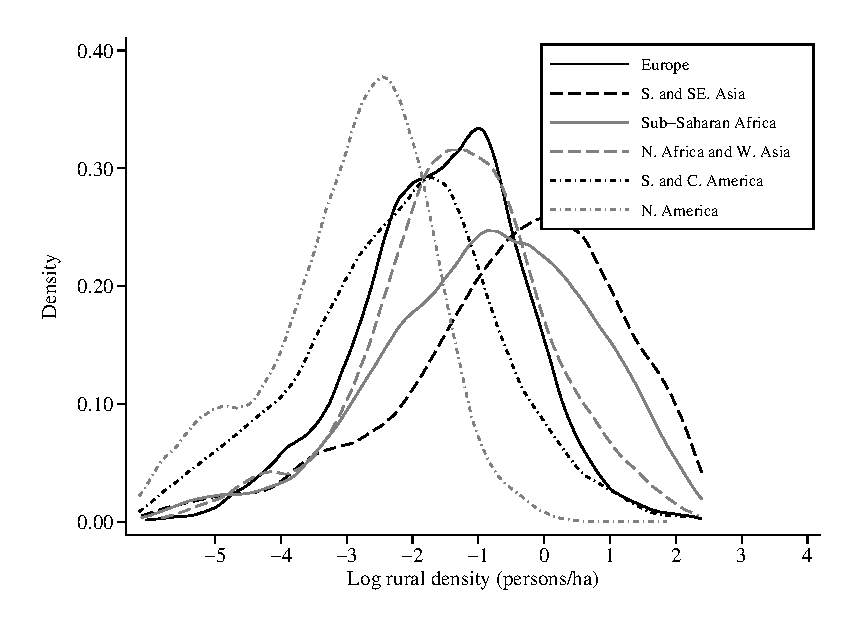
\includegraphics[width=1.0\textwidth]{fig_dens_rurd.eps}
\end{center}
\vspace{-.5cm}\singlespacing {\footnotesize \textbf{Notes}: Kernel density plot, Epanechnikov kernel, of the (log) rural density, $L_{Aisc}/X_{isc}$, at the district level, calculated by the authors using data from \citet{hyde31} for rural population. See text for details. See appendix for lists of exact countries included in each region.
}
\end{figure}

\clearpage

\begin{figure}[!htb]
\begin{center}
\caption{Density Plot of Caloric Yield ($A_{isc}$), by Region}
\label{FIG_dens_csi}
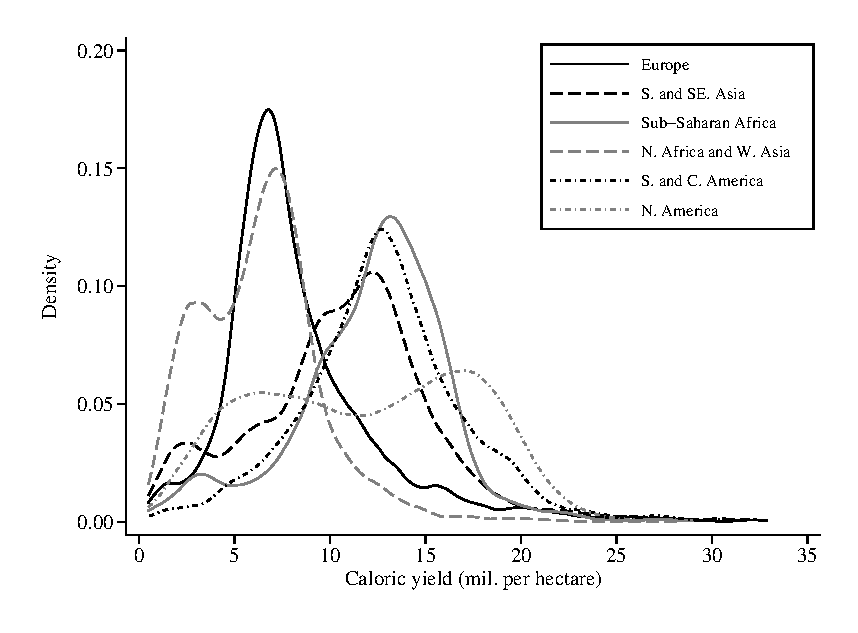
\includegraphics[width=1.0\textwidth]{fig_dens_csi.eps}
\end{center}
\vspace{-.5cm}\singlespacing {\footnotesize \textbf{Notes}: Kernel density plot, Epanechnikov kernel, of the caloric yield, $A_{isc}$, at the district level, calculated by the authors using data from \citet{galorozak2016}. See text for details. This measure sums the maximum calories available per grid cell within a district, then divides by total area of the district. See appendix for lists of exact countries included in each region.
}
\end{figure}

\clearpage

\begin{table}[!htb]
\begin{center}
\caption{Summary Statistics for District Level Data, 2000CE}
\label{TAB_summ}
{\small
\begin{tabularx}{\textwidth}{lXXXXXXX}
\midrule
 &      &            & \multicolumn{5}{c}{Percentiles:} \\ \cmidrule{4-8}
 & Mean & SD  & 10th    & 25th    & 50th & 75th & 90th \\
\midrule
Labor/land (persons/ha) &     0.73&     1.17&     0.04&     0.12&     0.32&     0.77&     1.86\\
Caloric yield (mil cals/ha) &    10.85&     4.89&     4.98&     7.17&    10.65&    13.86&    17.03\\
Log light density &    -2.82&     2.93&    -6.14&    -3.83&    -2.51&    -0.89&     0.35\\

\midrule
\end{tabularx}
}
\end{center}
\vspace{-.5cm}\singlespacing {\footnotesize \textbf{Notes}: A total of\districts \ observations for each variable (these come from\provinces \ provinces in\countries \ countries). Caloric yield, $A_{isc}$ calculated by the authors using data from \citet{galorozak2016}. Rural density, $L_{Aisc}/X_{isc}$ calculated by the authors using data from \citet{hyde31} for rural population. Both caloric yield and rural density were trimmed at the 99th and 1st percentiles of their raw data prior to calculating the summary statistics in this table. Urbanization rate taken from \citet{hyde31}. Log mean light density derived from the Global Radiance Calibrated Nightime Lights data provided by NOAA/NGDC, as in \citet{hssw2016}. 
}
\end{table}

\clearpage

\begin{table}[!htb]
\begin{center}
\caption{Estimates of Malthusian Tightness, $\beta$, by Agriculture Type, 2000CE}
\label{TAB_beta_crops}
{\footnotesize
\begin{tabularx}{\textwidth}{lXXXXXX}
\midrule
\multicolumn{7}{l}{Dependent Variable in all panels: Log caloric yield ($A_{isg}$)} \\ \\
\multicolumn{7}{l}{Panel A: Regions defined by:} \\ \\
 & \multicolumn{2}{c}{Suitability:} & \multicolumn{2}{c}{Max calories:} & \multicolumn{2}{c}{Harvest area:}\\ \cmidrule(lr){2-3} \cmidrule(lr){4-5} \cmidrule(lr){6-7} 
 & Temperate & Tropical & Temperate  & Tropical  & Temperate  & Tropical \\
 & (1) & (2) & (3) & (4) & (5) & (6) \\
\midrule
Log labor/land ratio ($\beta_g$)&       0.239&       0.088&       0.218&       0.093&       0.220&       0.081\\
                    &     (0.045)&     (0.020)&     (0.039)&     (0.012)&     (0.049)&     (0.016)\\
\midrule
p-value $\beta_g=0$ &       0.000&       0.000&       0.000&       0.000&       0.000&       0.000\\
p-value $\beta_g=\beta_{Temp}$&            &       0.002&            &       0.002&            &       0.007\\
Countries           &          84&          76&          91&         101&          86&          78\\
Observations        &        9404&        7229&       15260&       14794&       10221&       10013\\
R-square (ex. FE)   &        0.24&        0.20&        0.21&        0.18&        0.23&        0.18\\

\midrule
\\
\multicolumn{7}{l}{Panel B: With other restrictions (using suitability to define temperate/tropical)} \\ \\
 & \multicolumn{2}{c}{Urban Pop. $<25K$:} & \multicolumn{2}{c}{Ex. Europe/N. Amer.:} & \multicolumn{2}{c}{Rural dens. $>$ 25th P'tile:}\\ \cmidrule(lr){2-3} \cmidrule(lr){4-5} \cmidrule(lr){6-7}
 & Temperate & Tropical & Temperate  & Tropical  & Temperate  & Tropical \\
 & (1) & (2) & (3) & (4) & (5) & (6) \\
\midrule
Residuals           &       0.257&       0.140&       0.223&       0.131&       0.215&       0.128\\
                    &     (0.022)&     (0.021)&     (0.032)&     (0.018)&     (0.021)&     (0.020)\\
\midrule
p-value $\beta=0$   &       0.000&       0.000&       0.000&       0.000&       0.000&       0.000\\
p-value $\beta=\beta_{Temp}$&            &       0.000&            &       0.009&            &       0.003\\
Countries           &          83&          75&          24&          70&          82&          66\\
Observations        &        7648&        6662&         824&        8826&        8084&        6611\\
Adjusted R-square   &        0.29&        0.24&        0.16&        0.14&        0.24&        0.20\\

\midrule
\end{tabularx}
}
\end{center}
\vspace{-.5cm}\singlespacing {\footnotesize \textbf{Notes}: Conley standard errors, adjusted for spatial auto-correlation with a cutoff distance of 500km, are shown in parentheses. All regressions include province fixed effects, a constant, and controls for the district urbanization rate and log density of district nighttime lights. The coefficient estimate on rural population density indicates the value of $\beta_g$, see equation (\ref{EQ_regress}). Rural population is from HYDE database \citep{hyde31}, and caloric yield is the author's calculations based on the data from \citet{galorozak2016}. Inclusion of districts in the regression is based on the listed criteria related to crop families. See text for details of how temperate and tropical regions are defined in each case.
}
\end{table}

\clearpage

\begin{table}[!htb]
\begin{center}
\caption{Estimates of Malthusian Tightness, $\beta$, by K{\"o}ppen-Geiger Zone, 2000CE}
\label{TAB_beta_kg}
{\footnotesize
\begin{tabularx}{\textwidth}{lXXXXXX}
\midrule
\multicolumn{7}{l}{Dependent Variable in all panels: Log caloric yield ($A_{isc}$)} \\ \\
\multicolumn{7}{l}{Panel A: Climate Zones} \\
 & Equatorial & Arid & Temperate & Snow  &     &   \\
 & (1) & (2) & (3) & (4) &  & \\
\midrule
Log rural density   &       0.111&       0.154&       0.169&       0.230\\
                    &     (0.015)&     (0.026)&     (0.017)&     (0.026)\\
\midrule
p-value $\beta=0$   &       0.000&       0.000&       0.000&       0.000\\
p-value $\beta=\beta^{Equa}$&            &       0.151&       0.007&       0.000\\
Countries           &          79&          56&          94&          40\\
Observations        &       11461&        2822&       13717&        6327\\
Adjusted R-square   &        0.11&        0.10&        0.15&        0.19\\

\midrule
\\
\multicolumn{7}{l}{Panel B: Precipitation Zones} \\
& Fully     & Dry         & Dry        &              &            & \\
& Humid & Summer & Winter & Monsoon & Desert & Steppe \\
 & (1) & (2) & (3) & (4) & (5) & (6) \\
\midrule
Log labor/land ratio ($\beta_g$)&       0.240&       0.215&       0.124&       0.125&       0.130&       0.147\\
                    &     (0.044)&     (0.063)&     (0.022)&     (0.039)&     (0.072)&     (0.029)\\
\midrule
p-value $\beta=0$   &       0.000&       0.001&       0.000&       0.001&       0.072&       0.000\\
p-value $\beta=\beta_{Humid}$&            &       0.739&       0.020&       0.043&       0.190&       0.072\\
Countries           &          78&          37&          67&          32&          20&          49\\
Observations        &       13545&        2373&        7695&        1267&         146&        1735\\
R-square (ex. FE)   &        0.17&        0.17&        0.15&        0.17&        0.17&        0.16\\

\midrule
\\
\multicolumn{7}{l}{Panel C: Temperature Zones} \\
    & Hot        & Warm        & Cool       & Hot      & Cold     &  \\
    & Summer & Summer & Summer & Arid & Arid &   \\
 & (1) & (2) & (3) & (4) & (5) &  \\    
\midrule
Log labor/land ratio ($\beta_g$)&       0.142&       0.226&       0.207&       0.140&       0.190\\
                    &     (0.021)&     (0.053)&     (0.076)&     (0.035)&     (0.046)\\
\midrule
p-value $\beta=0$   &       0.000&       0.000&       0.007&       0.000&       0.000\\
p-value $\beta=\beta_{Humid}$&            &       0.065&       0.405&       0.969&       0.254\\
Countries           &          57&          82&          18&          42&          25\\
Observations        &        8101&        9003&         340&        1230&         956\\
R-square (ex. FE)   &        0.20&        0.23&        0.20&        0.17&        0.21\\

\midrule
\end{tabularx}
}
\end{center}
\vspace{-.5cm}\singlespacing {\footnotesize \textbf{Notes}: Conley standard errors, adjusted for spatial auto-correlation with a cutoff distance of 500km, are shown in parentheses. All regressions include province fixed effects, a constant, and controls for the district urbanization rate and log density of district nighttime lights. The coefficient estimate on rural population density indicates the value of $\beta$, see equation (\ref{EQ_regress}). Rural population is from HYDE database \citep{hyde31}, and caloric yield is the author's calculations based on the data from \citet{galorozak2016}. Inclusion of districts is based on whether they have more than 50\% of their land area in the given K{\"o}ppen-Geiger zone. See text for details.
}
\end{table}

\clearpage
\begin{table}[!htb]
\begin{center}
\caption{Estimates of Malthusian Tightness, $\beta$, by Regions, 2000CE}
\label{TAB_beta_subregion}
{\footnotesize
\begin{tabularx}{\textwidth}{lXXXXX}
\midrule
\multicolumn{6}{l}{Dependent Variable in all panels: Log caloric yield ($A_{isc}$)} \\ \\
\multicolumn{6}{l}{Panel A} \\
 &          &         &             &  \multicolumn{2}{c}{Excl. China, Japan, Korea} \\ \cmidrule(lr){5-6}
 & North \& &         &              & South \&  & Central \&             \\
 & Western  & Eastern & Southern     & Southeast & West        \\
 & Europe   & Europe  & Europe       & Asia      & Asia      \\
 & (1) & (2) & (3) & (4) & (5) \\
\midrule
Log rural density ($\beta_g$)&       0.259&       0.287&       0.272&       0.152&       0.181\\
                    &     (0.036)&     (0.031)&     (0.041)&     (0.026)&     (0.024)\\
\midrule
p-value $\beta=0$   &       0.000&       0.000&       0.000&       0.000&       0.000\\
p-value $\beta=\beta_{NWEur}$&            &       0.539&       0.791&       0.017&       0.072\\
Countries           &          16&           9&           9&          13&          18\\
Observations        &        1684&        4821&        1137&        4312&        2878\\
R-square (ex. FE)   &        0.29&        0.34&        0.32&        0.21&        0.24\\

\midrule
\\
\multicolumn{6}{l}{Panel B} \\
 & Temperate & Tropical  & Tropical & South    & North    \\
 & Americas  & Americas  & Africa   & Africa   & Africa     \\
\midrule
Residuals           &       0.188&       0.113&       0.089&       0.134&       0.249\\
                    &     (0.030)&     (0.016)&     (0.014)&     (0.071)&     (0.014)\\
\midrule
p-value $\beta=0$   &       0.000&       0.000&       0.000&       0.059&       0.000\\
p-value $\beta=\beta_{NWEur}$&       0.133&       0.000&       0.000&       0.116&       0.827\\
Countries           &           5&          22&          39&           4&           5\\
Observations        &        3796&        9373&        3181&         198&        1220\\
R-square (ex. FE)   &        0.24&        0.12&        0.18&        0.27&        0.28\\

\midrule
\\
\multicolumn{6}{l}{Panel C} \\
 & All& Temperate & Sub-Tropical & & North \& \\
 & China & China  & China & Japan & South Korea  \\
 & (1) & (2) & (3) & (4) & (5) \\
\midrule
Log rural density   &       0.414&       0.518&       0.107&       0.155&       0.190\\
                    &     (0.083)&     (0.058)&     (0.026)&     (0.011)&     (0.061)\\
\midrule
p-value $\beta=0$   &       0.000&       0.000&       0.000&       0.000&       0.002\\
p-value $\beta=\beta^{NWEur}$&       0.102&       0.000&       0.001&       0.008&       0.309\\
Countries           &           1&           1&           1&           1&           2\\
Observations        &         266&         130&         136&        1039&         311\\
Adjusted R-square   &        0.25&        0.26&        0.21&        0.21&        0.21\\

\midrule

\end{tabularx}
}
\end{center}
\vspace{-.5cm}\singlespacing {\footnotesize \textbf{Notes}: Conley standard errors, adjusted for spatial auto-correlation with a cutoff distance of 500km, are shown in parentheses. All regressions include province fixed effects, a constant, and controls for the district urbanization rate and log density of district nighttime lights. See appendix for lists of exact countries included in each region. The coefficient estimate on rural population density indicates the value of $\beta$, see equation (\ref{EQ_regress}). Rural population is from HYDE database \citep{hyde31}, and caloric yield is the author's calculations based on the data from \citet{galorozak2016}. The countries included in each region can be found in the appendix.
}
\end{table}

\clearpage
\begin{table}[!htb]
\begin{center}
\caption{Panel Estimates of Effect of Population Change, by Tightness of Malthusian Constraint}
\label{TAB_pop_panel}
{\footnotesize
\begin{tabularx}{\textwidth}{lXXXXXX}
\midrule
 & \multicolumn{6}{c}{Dependent Variable:} \\ \cmidrule(lr){2-7}
 & \multicolumn{2}{c}{Log GDP per capita} & \multicolumn{2}{c}{Log GDP per worker} & \multicolumn{2}{c}{Log population} \\ \cmidrule(lr){2-3} \cmidrule(lr){4-5} \cmidrule(lr){6-7}
 & Loose          & Tight          & Loose          & Tight          & Loose          & Tight \\
 & $\beta<$Median & $\beta>$Median & $\beta<$Median & $\beta>$Median & $\beta<$Median & $\beta>$Median \\
 & (1) & (2) & (3) & (4) & (5) & (6) \\
\midrule
 & \multicolumn{6}{c}{Panel A:} \\ \cmidrule(lr){2-7}
Mortality rate      &       0.333&       0.723&       0.284&       0.776&      -0.361&      -0.597\\
                    &     (0.271)&     (0.136)&     (0.262)&     (0.145)&     (0.186)&     (0.152)\\
\midrule
p-value $\theta=0$  &       0.220&       0.000&       0.281&       0.000&       0.054&       0.000\\
p-value $\theta=\theta^{Loose}$&           .&       0.199&           .&       0.102&           .&       0.327\\
Countries           &          16&          16&          16&          16&          16&          16\\
Observations        &         128&         128&         128&         128&         128&         128\\

\midrule
\\
 & \multicolumn{6}{c}{Panel B:} \\ \cmidrule(lr){2-7}
Log life expectancy &       0.309&      -2.007&       0.214&      -1.928&       1.910&       1.564\\
                    &     (0.393)&     (0.308)&     (0.387)&     (0.309)&     (0.235)&     (0.229)\\
\midrule
p-value $\theta=0$  &       0.434&       0.000&       0.582&       0.000&       0.000&       0.000\\
p-value $\theta=\theta^{Below}$&           .&       0.000&           .&       0.000&           .&       0.292\\
Countries           &          13&          14&          13&          14&          13&          14\\
Observations        &          99&         106&          99&         106&          99&         106\\

\midrule
\\
 & \multicolumn{6}{c}{Panel C:} \\ \cmidrule(lr){2-7}
Log population      &      -0.380&      -0.776&      -0.383&      -0.763\\
                    &     (0.125)&     (0.067)&     (0.121)&     (0.062)\\
\midrule
p-value $\theta=0$  &       0.003&       0.000&       0.002&       0.000\\
p-value $\theta=\theta^{Below}$&           .&       0.006&           .&       0.006\\
Countries           &          16&          16&          16&          16\\
Observations        &         128&         128&         128&         128\\

\midrule
\end{tabularx}
}
\end{center}
\vspace{-.5cm}\singlespacing {\footnotesize \textbf{Notes}: Robust standard errors are reported in parentheses. All regressions include both year fixed effects and country fixed effects. The value of $\beta$ for each country was found by estimating equation (\ref{EQ_regress}) separately for each, including province-level fixed effects. Countries are then included in a regression here based on how their $\beta$ compares to the median from the 32 countries, with those below the median denoted ``loose'', and those above the median denoted ``tight''. The mortality rate used as an explanatory variable in Panel A is the mortality rate from 15 infectious diseases, as documented by \cite{aj07}. All data on GDP per capita, GDP per worker, population, and life expectancy is also taken from those author's dataset. The p-value of $\theta = \theta^{Loose}$ is from a test that the estimated coefficient in a column for countries with ``tight'' constraints is equal to the coefficient in the column immediately preceding, using countries with ``loose'' constraints.
}
\end{table}



\end{document}